\section{BGK, AWBS, and Fokker-Planck models in local diffusive regime}
\label{sec:DiffusiveKinetics}

In a~broad analysis of the~electron transport, any qualitative information
about its properties are highly welcome. Even better, if one can extract some 
qualitative information, which provides comparative and reliable results in 
a~clear way, the~confidence of using a~transport model, 
e.g. \eqref{eq:AWBS_model}, can lead to efficient yet relatively
cheap computation cost predictions of real physics.

In this paper, we can try to find an~approximate solution to the~so-called
\textit{local diffusive regime} of electro transport, 
where the~\textit{diffusive regime}, in general, refers to a~low anisotropy 
in angle given by $\mu$, and \textit{local} means that the~mean free path of 
electrons $\mfpei$ is rather restricted compared to the~plasma spatial scale. 
In the~words of mathematics this corresponds to the~first 
order expansion in $\mfpei$ and $\mu$ of the~distribution function as
\begin{equation}
  \tilde{\ft}(z, \vmag, \mu) = \ft^0(z, \vmag) + \ft^1(z, \vmag) \mfpei\mu ,
  \label{eq:f_approximation}
\end{equation}
where $z$ is the~spatial coordinate along the~axis $z$, $\vmag$ the~magnitude 
of transport velocity, and 
$\mfpei = \frac{\vmag}{\nuei} = \frac{\vmag^4}{\Zbar n_e \Gamma}$.
In other words, one can say that by evaluating numerically $\tilde{\ft}$
in \eqref{eq:f_approximation}, we accept some error of the~order 
$O(\mfpei^2) + O(\mu^2)$. The~expansion in a~small parameter $\mfpei$ is also
coherent with a~time-steady approximation due to the~relation between the~mean
free path and collision frequency, where the~higher the~collision frequency 
the~more steady the~solution. 

In order to start, we express the~time-steady left hand side of 
\eqref{eq:kinetic_equation}
in 1D and insert the~approximation \eqref{eq:f_approximation}, which leads to
\begin{multline}
  \mu\left(\pdv{\tilde{f}}{z} + \frac{\tEz}{\vmag}\pdv{\tilde{f}}{\vmag}\right) 
  + \frac{\tEz(1-\mu^2)}{\vmag^2}\pdv{\tilde{f}}{\mu} = \\
  \mu\left(\pdv{f^0}{z} + \frac{\tEz}{\vmag}\pdv{f^0}{\vmag}\right) 
  + \frac{\tEz\mfpei}{\vmag^2} f^1 + O(\mu^2) ,
  \label{eq:LHS_kinetic_equation}
\end{multline}
and is truncated for low anisotropy, i.e. with error $O(\mu^2)$.

\subsection{The~BGK local diffusive electron transport}
\label{sec:BGKDiffusiveRegime}

Even though the~BGK plasma collisional operator \cite{BGK_1954}
\begin{equation}
  \frac{1}{\vmag}C_{BGK}(\tilde{\ft})
  =
  \frac{\tilde{\ft} - \fM}{\mfpe}
  + \frac{1}{2 \mfpei}
  \pdv{}{\mu}(1 - \mu^2)\pdv{\tilde{\ft}}{\mu} ,
  \label{eq:BGK_model_1D}
\end{equation}
where $\mfpe = \Zbar \mfpei$, 
is not actually used in our nonlocal transport simulations, we consider it 
useful to include this~simplest form of the~Boltzmann transport collision 
operator, because of two reasons: a) it can be treated analytically in 
the~local diffusive regime; and b) it represents the~so-called phenomenological
collision operator by explicitly using the~Maxwell-Boltzmann equilibrium 
distribution $\fM$, which proves to be very useful in coupling of the~nonlocal 
electron transport to hydrodynamics.

If one applies the~action of the~right hand side, i.e. of 
\eqref{eq:BGK_model_1D}, 
on the~approximation \eqref{eq:f_approximation} and sets the~result to be equal 
to the~left hand side \eqref{eq:LHS_kinetic_equation}, the~corresponding terms
in $\mu$ are governed by the~following equations
\begin{eqnarray}
  \ft^0 &=& \fM + \frac{\tEz}{\vmag^2}f^1 \Zbar\mfpei^2 ,
  \label{eq:BGK_f0} \\
  \ft^1 &=& - \frac{\Zbar}{\Zbar+1}
  \left( \pdv{\ft^0}{z} + \frac{\tilde{E}_z}{\vmag}\pdv{\ft^0}{\vmag} \right) , 
  \label{eq:BGK_f1}
\end{eqnarray}
i.e. $\ft^0 = \fM + O(\mfpei^2)$ and $\ft^1 = - \frac{\Zbar}{\Zbar+1}
  \left( \pdv{\fM}{z} + \frac{\tilde{E}_z}{\vmag}\pdv{\fM}{\vmag} \right)$.
%\begin{equation}
%  \tilde{f} = \fM - \frac{\Zbar}{\Zbar+1}
%  \left(\frac{1}{\rho}\pdv{\rho}{z} + 
%  \left( \frac{\vmag^2}{2 \vth^2} - \frac{3}{2}\right)
%  \frac{1}{T}\pdv{T}{z} - \frac{\tilde{E}_z}{\vth^2} \right)\fM \mfpei \mu , 
%  \nonumber
%\end{equation}
Now the~electric current expressing the~contribution of every electron 
naturally tends to zero, i.e. the~\textit{quasi-neutrality} constraint, 
which lead to an~analytic formula of the~self-consistent electric field
\begin{multline}
\vect{j} \equiv \qe \int \vv \tilde{\ft} \, \dI\vv = \vect{0}  \rightarrow
\tE = \vth^2\left(\frac{\nabla\rho}{\rho} + \frac{5}{2}\frac{\nabla T}{T} 
\right) .
\label{eq:BGK_Efield}
\end{multline}
Consequently, based on \eqref{eq:BGK_f0}, \eqref{eq:BGK_f1}, 
and \eqref{eq:BGK_Efield}, the~analytic formula \eqref{eq:f_approximation}
of the~electron distribution function reads 
\begin{equation}
  \tilde{f} = \fM - \frac{\Zbar}{\Zbar+1}
  \left( \frac{\vmag^2}{2 \vth^2} - 4\right)
  \frac{1}{T}\pdv{T}{z}\fM \mfpei \mu , 
  \label{eq:BGK_approximation}
\end{equation}
which is nothing else than the~famous Lorentz electron-ion collision gas model 
\cite{Lorentz_1905} scaled by a~constant depending on $\Zbar$, 
naturally arising from the~BGK model \eqref{eq:BGK_model_1D}.

\subsection{The~AWBS local diffusive electron transport}
\label{sec:AWBSDiffusiveRegime}
The~main object of this work presented in Sec~\ref{sec:AWBSmodel} simplifies
in 1D to a~relatively simple form of the~Boltzmann transport collision operator
(compared to \eqref{eq:LFP_model})
\begin{multline}
  \frac{1}{\vmag}C_{AWBS}(f)
  = 
  \frac{\vmag}{2\mfpe} \pdv{}{\vmag}\left(f - \fM\right) \\
  + \frac{1}{2}\left(\frac{1}{\mfpei} + \frac{1}{2\mfpe}\right)
  \pdv{}{\mu}(1 - \mu^2)\pdv{f}{\mu} .
  \label{eq:AWBS_model_1D}
\end{multline}
Similarly to the~BGK model, AWBS \ref{eq:AWBS_model_1D} 
is also referred to as a~phenomenological model, since it explicitly uses 
the~Maxwell-Boltzmann equilibrium distribution $\fM$, and also, 
makes it a~very attractive model of the~nonlocal electron
transport to be coupled to hydrodynamics via the~plasma electron temperature 
and density.

A~qualitative information about the~AWBS model is obtained while repeating
the~action on \eqref{eq:f_approximation} by the~left hand side 
\eqref{eq:LHS_kinetic_equation} and by the~right hand side 
\eqref{eq:AWBS_model_1D} and setting the~equality. The~corresponding terms
in $\mu$ are then governed by the~following equations
\begin{eqnarray}
  \pdv{}{\vmag}\left( f^0 -\fM\right) &=& 
  \frac{\tEz}{\vmag^3}f^1 2\Zbar\mfpei^2 ,
  \label{eq:AWBS_f0} \\
  \frac{\vmag}{2\Zbar\mfpei}\pdv{\left(f^1 \mfpei\right)}{\vmag}  
  - \frac{2\Zbar + 1}{2\Zbar} f^1 &=&
  \pdv{f^0}{z} + \frac{\tilde{E}_z}{\vmag}\pdv{f^0}{\vmag} ,
  \label{eq:AWBS_f1} 
  %\\  
  %\frac{\vmag}{\Zbar}\pdv{f^1}{\vmag} + \frac{4}{\Zbar}f^1 
  %- \frac{\Zbar + 1}{\Zbar} f^1 &=&
  %\pdv{f^0}{z} + \frac{\tilde{E}_z}{\vmag}\pdv{f^0}{\vmag}
  %\nonumber
\end{eqnarray}
i.e. $\ft^0 = \fM + O(\mfpei^2)$, however, the~$\ft^1$ does not have 
a~straightforward analytic formula. In reality, $\ft^1$ arises from 
the~ordinary differential equation 
(by inserting $\fM$ into \eqref{eq:AWBS_f1})
\begin{multline}
  \pdv{f^1}{\vmag} + \frac{1}{\vmag}(3-2\Zbar)f^1
  = \\
  \frac{2\Zbar}{\vmag}\left(\frac{1}{\rho}\pdv{\rho}{z} + 
  \left( \frac{\vmag^2}{2 \vth^2} - \frac{3}{2}\right)
  \frac{1}{T}\pdv{T}{z} - \frac{\tilde{E}_z}{\vth^2}\right)\fM .
  \label{eq:AWBS_f1_ODE}
\end{multline}
We will stick with a~numerical solution of \eqref{eq:AWBS_f1_ODE}, where
the~details about the~resulting distribution function can be found in 
Section~\ref{sec:SummaryDiffusiveKinetics}. 

\subsection{The~Fokker-Planck local diffusive electron transport}
\label{sec:FPDiffusiveRegime}
\newcommand{\gt}{g}
\newcommand{\gM}{\gt_M}

The~Fokker-Plank \eqref{eq:LFP_model} collision operator can be also written as 
\cite{Shkarofsky_Particle_Kinetics_book_1966_24}
\begin{equation}
  \frac{1}{\vmag}C_{FP}(f) =  
  \frac{\Gamma}{\vmag} \left(4\pi f^2 
  + \frac{\gv\gv \ft : \gv\gv \gt}{2}\right) ,
  \label{eq:FP_model_1D}
\end{equation}
where $g(\vv) = \int |\vv - \vvb| f(\vvb)\, \dI\vvb$ is 
the~Rosenbluth potential \cite{Rosenbluth_PR1957}. Since we are interested in 
the~approximate solution in the~local diffusive regime, it is convenient to
use a~low anisotropy approximation 
$\tilde{\gt} = \gt^0(f^0) + \gt^1(f^1) \mfpei \mu$, which arises based on 
Eq. 45 of \cite{Rosenbluth_PR1957}.

For a~better clarity we present the~action of \eqref{eq:FP_model_1D} in 1D
\begin{multline}
  C_{FP}(\tilde{f}) = 
  \Gamma\left(4\pi{\ft^0}^2 + 
  \frac{1}{2}\frac{\partial^2 \ft^0}{\partial \vmag^2}
  \frac{\partial^2 \gt^0}{\partial \vmag^2}
  + \frac{1}{\vmag^2}\pdv{\ft^0}{\vmag}\pdv{\gt^0}{\vmag} \right)
  \\
  + \frac{\mu}{\Zbar n_e}
  \Bigg[8\pi \ft^0 \ft^1\vmag^4 - \vmag\left(\pdv{\ft^0}{\vmag}\gt^1
  + \pdv{\gt^0}{\vmag}\ft^1\right) 
  \\
  + \frac{1}{\vmag^2}\left(\pdv{\ft^0}{\vmag}
  \pdv{(\gt^1\vmag^4)}{\vmag}
  + \pdv{\gt^0}{\vmag}\pdv{(\ft^1\vmag^4)}{\vmag}\right) \\
  + \frac{1}{2}\left(\frac{\partial^2 \ft^0}{\partial \vmag^2}
  \frac{\partial^2 (\gt^1\vmag^4)}{\partial \vmag^2}
  + \frac{\partial^2 \gt^0}{\partial \vmag^2} 
  \frac{\partial^2 (\ft^1\vmag^4)}{\partial \vmag^2}
  \right) \Bigg] + O(\mfpei^2, \mu^2) ,
  \label{eq:FP_truncation}
\end{multline}
truncated by the~quadratic terms in the~angular anisotropy and the~transport 
localization.
%where the~isotropic contribution $O(\mfpei^2) = \frac{2}{\vmag^2}
%  \left(\pdv{\ft^1\mfpei}{\vmag} - \frac{\ft^1\mfpei}{\vmag} \right)
%  \left(\pdv{\gt^1\mfpei}{\vmag} - \frac{\gt^1\mfpei}{\vmag} \right)$.

If once more repeated the~action on \eqref{eq:f_approximation} by the~left 
hand side \eqref{eq:LHS_kinetic_equation} and by the~right hand side 
\eqref{eq:FP_model_1D} and setting the~equality, the~equation governing
$\ft^0$ corresponding to $\mu^0$ takes the~form
\begin{multline}
  4\pi{\ft^0}^2 + 
  \frac{1}{2}\frac{\partial^2 \ft^0}{\partial \vmag^2}
  \frac{\partial^2 \gt^0}{\partial \vmag^2}
  + \frac{1}{\vmag^2}\pdv{\ft^0}{\vmag}\pdv{\gt^0}{\vmag} = 
  \frac{\tEz}{\vmag^5}f^1 \Zbar n_e\mfpei^2 \\
  - \frac{2}{\vmag^2}
  \left(\pdv{\ft^1\mfpei}{\vmag} - \frac{\ft^1\mfpei}{\vmag} \right)
  \left(\pdv{\gt^1\mfpei}{\vmag} - \frac{\gt^1\mfpei}{\vmag} \right),
  \label{eq:FP_f0} 
\end{multline}
where the~fundamental property of the~Fokker-Planck collision operator
tending to the~Maxwell-Boltzmann distribution $\fM$ \cite{Longmire_1963}, leads
to $\ft^0 = \fM + O(\mfpei^2)$, where we write an~explicit form of 
the~quadratic term $O(\mfpei^2)$ obtained from the~truncation 
\eqref{eq:FP_truncation}.
%\begin{multline}
%  \frac{1}{2}\left(\frac{\partial^2 \ft^0}{\partial \vmag^2}
%  \frac{\partial^2 (\gt^1\vmag^4)}{\partial \vmag^2}
%  + \frac{\partial^2 \gt^0}{\partial \vmag^2} 
%  \frac{\partial^2 (\ft^1\vmag^4)}{\partial \vmag^2}
%  \right) 
%  + \frac{1}{\vmag^2}\left(\pdv{\ft^0}{\vmag} \pdv{(\gt^1\vmag^4)}{\vmag} 
%  + \pdv{\gt^0}{\vmag}\pdv{(\ft^1\vmag^4)}{\vmag}\right) \\
%  - \vmag\left(\pdv{\ft^0}{\vmag}\gt^1 
%  + \pdv{\gt^0}{\vmag}\ft^1\right)
%  + 8\pi \ft^0 \ft^1\vmag^4 
%  - \vmag \ft^1
%  = 
%  \vmag\pdv{f^0}{z} + \tilde{E}_z\pdv{f^0}{\vmag}
%  ,
%  \label{eq:FP_f1}
%\end{multline}
The~equality corresponding to $\mu$ takes the~form
\begin{multline}
  \frac{1}{\Zbar n_e}\Bigg[
  \frac{1}{2}\left(\frac{\partial^2 \fM}{\partial \vmag^2}
  \frac{\partial^2 (\gt^1\vmag^4)}{\partial \vmag^2}
  + \frac{\partial^2 \gM}{\partial \vmag^2} 
  \frac{\partial^2 (\ft^1\vmag^4)}{\partial \vmag^2}
  \right) \\ 
  + \frac{1}{\vmag^2}\left(\pdv{\fM}{\vmag} \pdv{(\gt^1\vmag^4)}{\vmag} 
  + \pdv{\gM}{\vmag}\pdv{(\ft^1\vmag^4)}{\vmag}\right) \\
  - \vmag\left(\pdv{\fM}{\vmag}\gt^1 
  + \pdv{\gM}{\vmag}\ft^1\right)
  + 8\pi \fM \ft^1\vmag^4 \Bigg]
  - \vmag \ft^1
  \\ =  
  %\vmag\left(\frac{1}{\rho}\pdv{\rho}{z} + 
  %\left( \frac{\vmag^2}{2 \vth^2} - \frac{3}{2}\right)
  %\frac{1}{T}\pdv{T}{z} - \frac{\tilde{E}_z}{\vth^2}\right)\fM
  \vmag\pdv{\fM}{z} + \tilde{E}_z\pdv{\fM}{\vmag} ,
  \label{eq:FP_f1_ODE}
\end{multline}
which is the~equation governing the~unknown $\ft^1$.

In principle, the~solution to the~equation \eqref{eq:FP_f1_ODE}
is very ambitious, as demonstrated in 
\cite{Chandrasekhar_RMP1943, CSR_1950, Rosenbluth_PR1957}, fortunately, one 
can use the~explicit evaluation of the~electron distribution function
published in \cite{SpitzerHarm_PR1953}, which takes the~following form
%The~Rosenbluth equation \refeq{eq:FP_Rosenbluth} can be further rewritten
%according to $[$Longmire, Conrad L. : Elementary Plasma Physics. Intersci. Pub., 1963$]$ as
%\begin{equation}
%  \left(\pdv{\ft}{t}\right)_c = \Gamma 4\pi f^2 
%  + \frac{\gv\gv\Rgb : \gv\gv \ft}{2} ,
%  \label{eq:FP_Longmire}
%\end{equation}
%which was also published in Shkarofsky 1966 and used in Tzoufras 2011.
\begin{comment} % FP appendix
\begin{equation}
  \vtwoh = \sqrt{\frac{2 \kB T}{\me}} = 1 / j,
  \nonumber
\end{equation}
\begin{eqnarray}
  A &=& -\frac{\me^2 \vtwoh^2 \tE}{2 \pi e^4 n_e \lnc} = - \frac{m E}{2\pi j^2 e^3 n_e \lnc}
  , \nonumber \\
  B &=& \frac{\me^2 \vtwoh^4 |\nabla T|}{2 \pi e^4 n_e \lnc T} = \frac{2 \kB^2 T |\nabla T|}{\pi e^4 n_e \lnc}
  , \nonumber
\end{eqnarray}
\begin{equation}
  \frac{A}{B} = - \frac{|\tE| T}{\vtwoh^2 |\nabla T|} ,
  \nonumber
\end{equation}
\begin{equation}
  \tE = -\frac{3}{2}\frac{\vtwoh^2}{2}\frac{\gamma_T}{\gamma_E}
  \frac{\nabla T}{T} ,
  \nonumber
\end{equation}
From Eq. (24) CSR, we can write the~form of $f_1$ including both $\nabla T$ 
and $\tE$ effects as
\begin{equation}
  f_1(\vmag, \theta) = \cos(\theta) \frac{B}{\Zbar}\left( d_T(\vmag/\vtwoh) 
  + \frac{A}{B} d_E(\vmag/\vtwoh) \right) \fM(\vmag)  ,
  \nonumber
\end{equation}
where in the~case of vanishing current one gets
\begin{equation}
  \frac{A}{B} = \frac{3}{2}\frac{\gamma_T}{2 \gamma_E} ,
  \nonumber
\end{equation}
i.e.
\end{comment} % FP appendix
\begin{multline}
  %\ft^1(\vmag, \mu) 
  \ft^1(z, \vmag) = \frac{1}{\mfpei}\frac{\me^2}{4 \pi \qe^4\lnc} 
  \frac{\vtwoh^4}{\Zbar}
  \\
  \left( 2 d_T(\vmag/\vtwoh) 
  + \frac{3}{2}\frac{\gamma_T}{\gamma_E} d_E(\vmag/\vtwoh) \right) 
  \frac{\fM}{n_e}\frac{1}{T}\pdv{T_e}{z}  ,
  \label{eq:f1_SH}
\end{multline}
where $d_T(x) = \Zbar D_{T}(x) / B$, $d_E(x) = \Zbar D_{E}(x) / A$, $\gamma_T$,
and $\gamma_E$ are represented by numerical values in TABLE~I, TABLE~II, and
TABLE~III in \cite{SpitzerHarm_PR1953}, and 
$\vtwoh = \sqrt{\frac{\kB T_e}{2\me}}$.

%In the~case of high $\Zbar$ limit, $\gamma_T \rightarrow 1$,
%$\gamma_E \rightarrow 1$, $d_E(x) = x^4$, and $d_T(x) = x^4 (2.5 - x^2)/2$
%\cite{SpitzerHarm_PR1953}, which leads to the~standard Lorentz gas model
%\begin{equation}
%   f_1(\vmag, \theta) = \cos(\theta) \frac{\me^2}{4 \pi e^4\lnc} 
%  \frac{\vmag^4}{\Zbar}\left( 4 - \frac{\vmag^2}{\vtwoh^2} \right) 
%  \frac{\fM(\vmag)}{n_e}\frac{\nabla T}{T}  ,
%  \label{eq:f1_Lorentz} 
%\end{equation} 

\subsection{Summary of the~BGK, AWBS, and Fokker-Planck local diffusive 
transport}
\label{sec:SummaryDiffusiveKinetics}

Ever since the~SH paper \cite{SpitzerHarm_PR1953}, the~effect of microscopic
electron transport on the~current $\int \qe \vv \tilde{\ft} \, \dI\vv$ 
and the~heat flux $\int \frac{\me |\vv|^2}{2} \vv \tilde{\ft} \, \dI\vv$ 
in plasmas
under local diffusive conditions has been understood. By overcoming some 
delicate aspects of the~numerical solution to \eqref{eq:FP_f1_ODE} presented 
in the~CSR paper \cite{CSR_1950}, the~effect of electron-electron collisions
was properly quantified and the~correct dependence on $\Zbar$ of the~heat flux
$\vect{q}$ was approximated as 
\begin{equation}
  \vect{q} = \frac{\Zbar + 0.24}{\Zbar + 4.2} \vect{q}_L ,
  \label{eq:qSH_approximation}
\end{equation}
where $\vect{q}_L = \kappa T_e^{\frac{5}{2}}\nabla T_e$ is the~heat flux given 
by Lorentz \cite{Lorentz_1905}.
In order to follow the~SH $\Zbar$-dependence of heat flux, the~BGK operator 
needs to be scaled as
\begin{equation}
  %C_{BGK}(\tilde{\ft})
  %=
  \frac{\Zbar + 4.2}{\Zbar + 0.24}
  \frac{\Zbar}{\Zbar+1}\left[\nue\left(\tilde{\ft} - \fM\right)
  + \frac{\nuei}{2}
  \pdv{}{\mu}(1 - \mu^2)\pdv{\tilde{\ft}}{\mu}\right] ,
  \nonumber
\end{equation}
which leads to a~scaled Lorentz$^*$ distribution function
\begin{equation}
  \tilde{f} = \fM - \frac{\Zbar+0.24}{\Zbar+4.2}
  \left( \frac{\vmag^2}{2 \vth^2} - 4\right)
  \frac{1}{T}\pdv{T}{z}\fM \mfpei \mu ,
  \label{eq:Scaled_Lorentz}
\end{equation}
which obeys the~$\Zbar$-dependence \eqref{eq:qSH_approximation}.

\begin{table}
\begin{center}
  \begin{tabular}{c|ccccc}
    \hline\hline\\
    %$\Zbar$ & $1$ & $2$ & $4$ & $16$ & $\infty$ \\\\
    & $\,\Zbar=1\,$ & $\,\Zbar=2\,$ & $\,\Zbar=4\,$ & $\,\Zbar=16\,$ & $\,\Zbar=116\,$ \\\\
    \hline\\
    $\bar{\Delta}\vect{q}_{AWBS}$ & 0.057 & 0.004 & 0.038 & 0.049 & 0.004 \\\\
    \hline\hline
  \end{tabular}
  \caption{
  Relative error $\bar{\Delta}\vect{q}_{AWBS} = 
  |\vect{q}_{AWBS} - \vect{q}_{SH}| / \vect{q}_{SH}$ of the~AWBS
  kinetic model equation \refeq{eq:AWBS_model} showing the~discrepancy 
  (maximum around 5$\%$) with respect to the~original solution of 
  the~heat flux given by numerical solution in Spitzer and Harm 
  \cite{SpitzerHarm_PR1953}.
  }
\label{tab:qAWBS}
\end{center}
\end{table}

On the~contrary, the~modified form of the~AWBS collision operator 
\eqref{eq:AWBS_model} provides a~very precise heat flux $\Zbar$-dependence
without introducing any scaling. Indeed, \tabref{tab:qAWBS} shows the~relative
error (maximum around 5$\%$) of the~heat flux modeled by 
\eqref{eq:AWBS_model} vs. SH results represented by 
\eqref{eq:qSH_approximation}. It should be noted that the~error is calculated 
with respect to original values presented in TABLE~III in 
\cite{SpitzerHarm_PR1953}.

Nevertheless, the~electron-electron collisions effect represented by 
\eqref{eq:qSH_approximation} provides only an~integrated information about
the~heat flux magnitude. If one takes a~closure look at the~distribution
function itself, the~conformity of the~modified AWBS collision operator
is even more emphasize as can be seen in \figref{fig:q1s_summary} showing
the~flux moment in spherical coordinates of velocity
\begin{equation}
  q_1 = \frac{\me\vmag^2}{2}\vmag \ft_1 \vmag^2 ,
  \nonumber
\end{equation}
where $\ft_1$ is the~anisotropic part of the~distribution function, i.e.
$\ft_1 = \ft^1\mfpei$ ($\mu=1$) in the~local diffusive transport.

In the~case of the~high $\Zbar$ Livermorium plasma ($\Zbar = 116$), 
AWBS exactly aligns with the~Lorentz gas limit. In the~opposite case of the~low
$\Zbar$ Hydrogen plasma ($\Zbar = 1$), the~AWBS distribution function 
approaches significantly the~numerical SH solution. Overall BGK behavior is 
consistent with the~scaled Lorentz$^*$ distribution function 
\eqref{eq:Scaled_Lorentz} for any $\Zbar$.  

\begin{figure}[tbh]
  \begin{center}
    \begin{tabular}{c}
      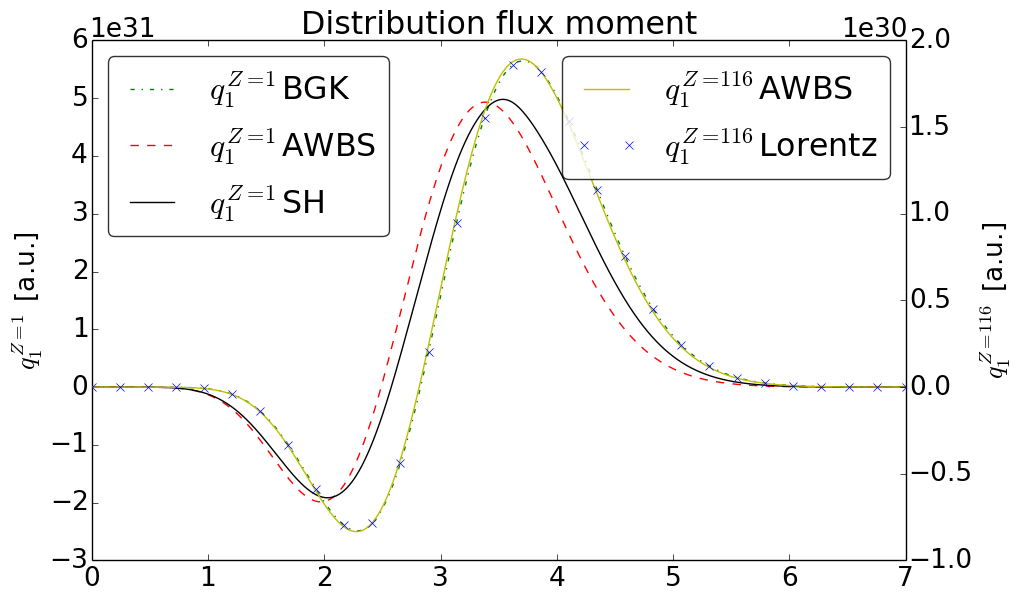
\includegraphics[width=0.5\textwidth]{q1s.png}
    \end{tabular}
  \caption{  
  The~flux velocity moment of the~anisotropic part of the~electron distribution 
  function in low $Z=1$ and high $Z=116$ plasmas in diffusive regime.}
  \label{fig:q1s_summary}
  \end{center} 
\end{figure}

If one observes the~$\ft^1$ equations of each of the~model, i.e.
\eqref{eq:BGK_f1}, \eqref{eq:AWBS_f1_ODE}, and \eqref{eq:FP_f1_ODE}, it turns
out to be clear that the~terms containing derivatives with respect to $\vmag$ 
address important physical mechanisms of electron-electron collisions in plasma.
In other words, even a~simple linear first derivative term in the~modified
AWBS collision operator \eqref{eq:AWBS_model} (red dashed line) provides 
a~significant model improvement with respect to the~SH (Fokker-Planck) solution
(solid black line) and compared to the~simplest BGK model
(dashed-dot blue line) in \figref{fig:q1s_summary}.

At last, we provide a~qualitative information with respect to the~dominant 
velocity of electrons contributing to the~heat flux. In the~high $\Zbar$ case
all the~models give 3.7$\times \vth$, while SH solution gives 3.5$\times \vth$
and AWBS 3.4$\times \vth$ in the~case of low $\Zbar$ plasmas, thus showing 
the~right tendency of the~maximum velocity shift modeled by the~modified AWBS
collision operator \eqref{eq:AWBS_model}.
%\begin{itemize} 
%  \item Point out the~behavior of the~maximum velocity of $q_1$, Lorentz 3.71, SHZ1 3.53, AWBSZ1 3.39.
%\end{itemize}

